\section{Mapping Rules for RDF-star: RML-star}
\label{sec:chp4_rml_star}

\ana{RAW TEXT FROM PAPER AHEAD}

\subsection{Statements about statements in mapping rules}
\label{sec:chp4_reif_mappings}

Making statements about statements in RDF
posed a challenge almost since the inception of RDF.
Indeed, the W3C RDF Primer~(\cite{manola2004rdf}) already included a description of the standard reification approach.
Other alternatives were proposed over the years,
such as singleton properties~(\cite{nguyen2014don}), RDF$^+$~(\cite{schueler2008querying}), and more recently, \mbox{RDF-star}~(\cite{hartig2017foundations}). 

This section describes popular reification approaches and shows how they can be used in RML and RML-star with a running example. 
Standard reification and singleton properties are considered in Section \ref{sec:chp4_validation}, showing that
\mbox{Morph-KGC$^{star}$} does not add any overhead in the time required to generate the \mbox{RDF-star} 
triples compared to them.

We illustrate each reification alternative with a running example that uses the data shown in Listing \ref{lst:csv}.
It contains CSV data related to pole vault:
the vaulter (\texttt{PERSON}),
the height of the jump (\texttt{MARK}),
the date when the jump was performed (\texttt{DATE}) and
an identifier of the jump (\texttt{ID}).
The running example represents
that a person jumped some height on a specific date, i.e., it adds the metadata about ``date''
to the statement ``a person jumped some height''.

\noindent\hspace{0.19\linewidth}\begin{minipage}{\linewidth}
\begin{captionedlisting}{lst:csv}{Contents of the logical source \texttt{:marks} in CSV format.}
\centering
\begin{tabular}{c}
\hspace{3em}
{\begin{lstlisting}[basicstyle=\ttfamily\small,label={list:example1},columns=flexible]
ID , DATE            , MARK ,   PERSON
1   , 2022-03-21 , 4.80 ,   Angelica
2   , 2022-03-19 , 4.85 ,   Katerina
\end{lstlisting}}
\end{tabular}
\end{captionedlisting}
\end{minipage}

\subsubsection{Reification with RML}

Two popular reification approaches exist: standard reification and singleton properties. 
These approaches use strategies that add metadata to triples
without additional constructs (e.g., named graphs~(\cite{hernandez2015reifying})).
They can be used with RML without any further modification. RML mapping rules enable the generation of blank nodes (required for standard reification) and dynamically generated predicates (required for singleton properties). 

\noindent\textbf{\textit{Standard Reification}}~(\cite{manola2004rdf}) was proposed in the W3C RDF Primer~(\cite{manola2004rdf}).
It assigns statements to unique identifiers (typically blank nodes) typed with \texttt{rdf:Statement} and described using the properties \texttt{rdf:subject}, \texttt{rdf:predicate} and \texttt{rdf:object}.
This way, the unique identifier representing the statement can be further annotated with additional statements. Listing \ref{lst:res-std-reif} shows an example of standard reification for the data in Listing \ref{lst:csv}, created with the RML mapping rules in Listing \ref{lst:std-reif}. 
This mapping creates blank nodes in the subject with the \texttt{ID} data field, typed with \texttt{rdf:Statement}; and has three predicate object maps to generate the \texttt{rdf:subject}, \texttt{rdf:predicate}, \texttt{rdf:object} of the triples and a predicate object map to annotate the statements with \texttt{:date}.

\noindent\textbf{\textit{Singleton Properties}}~(\cite{nguyen2014don}). This approach uses unique predicates linked with \texttt{rdf:singletonPropertyOf} to the original predicate. 
This unique predicate can then be annotated as the subject of additional statements. 
Listing \ref{lst:res-sp-reif} shows the reified triples for the data in Listing \ref{lst:csv} created with the RML mapping rules in Listing \ref{lst:sp-reif}. 
It uses a singleton property dynamically generated with the \texttt{ID} data field for the property \texttt{:jumps}, annotated with \texttt{:date}.


\begin{minipage}{0.45\linewidth}
\begin{captionedlisting}{lst:std-reif}{Example RML mapping using standard reification that transforms data in Listing \ref{lst:csv}.}
\centering
{\begin{lstlisting}[basicstyle=\ttfamily\small,label={list:example1},columns=flexible]
<#TM> a rr:TriplesMap ;
  rml:logicalSource :marks ;
  rr:subjectMap [ 
    rml:reference "ID" ;
    rr:termType rr:BlankNode ;
    rr:class rdf:Statement  ] ;
  rr:predicateObjectMap [ 
    rr:predicate rdf:subject ;
    rr:objectMap [
      rr:template ":{PERSON}" ] ] ;
  rr:predicateObjectMap [ 
    rr:predicate rdf:predicate ;
    rr:object :jumps ] ;
  rr:predicateObjectMap [ 
    rr:predicate rdf:object ;
    rr:objectMap [
      rml:reference "MARK" ] ] ;
  rr:predicateObjectMap [ 
    rr:predicate :date ;
    rr:objectMap [
      rml:reference "DATE" ] ] .
  
\end{lstlisting}}

\end{captionedlisting}
\end{minipage}
\,\,\,\,\hfill
\begin{minipage}{0.45\linewidth}
\begin{captionedlisting}{lst:sp-reif}{Example RML mapping using a singleton property that transforms data in Listing \ref{lst:csv}.}
\centering
{{\begin{lstlisting}[basicstyle=\ttfamily\small,label={list:example1},columns=flexible]
<#TM> a rr:TriplesMap ;
  rml:logicalSource :marks ;
  rr:subjectMap [ 
    rr:template ":{PERSON}" ] ;
  rr:predicateObjectMap [ 
    rr:predicateMap [
     rr:template ":jumps#{ID}" ] ;
    rr:objectMap [
      rml:reference "MARK" ] ] .
      
<#TM-SP> a rr:TriplesMap ;
  rr:logicalSource :marks ;
  rr:subjectMap [ 
    rr:template ":jumps#{ID}" ] ;
  rr:predicateObjectMap [ 
    rr:predicate rdf:singletonPropertyOf;
    rr:object :jumps ] ;
  rr:predicateObjectMap [ 
    rr:predicate :date ;
    rr:objectMap [
      rml:reference "DATE" ] ] .
\end{lstlisting}}}
\end{captionedlisting}
\end{minipage}




\begin{minipage}{0.42\linewidth}
\begin{captionedlisting}{lst:res-std-reif}{RDF triples generated by the mapping in Listing \ref{lst:std-reif}.}
\centering
{\begin{lstlisting}[basicstyle=\ttfamily\small,label={list:example1},columns=flexible]
_:1 rdf:type      rdf:Statement .
_:1 rdf:subject   :Angelica .
_:1 rdf:predicate :jumps .
_:1 rdf:object    "4.80" .
_:1 :date         "2022-03-21" .
_:2 rdf:type      rdf:Statement .
_:2 rdf:subject   :Katerina .
_:2 rdf:predicate :jumps .
_:2 rdf:object    "4.85" .
_:2 :date         "2022-03-19" .
\end{lstlisting}}
\end{captionedlisting}
\end{minipage}
\,\,\,\,
\begin{minipage}{0.5\linewidth}
\begin{captionedlisting}{lst:res-sp-reif}{RDF triples generated by the mapping in Listing \ref{lst:sp-reif}.}
\centering
{\begin{lstlisting}[basicstyle=\ttfamily\small,label={list:example1},columns=flexible]

:Angelica   :jumps#1            "4.80" .
:jumps#1    :date               "2022-03-21" .
:jumps#1    rdf:singletonPropertyOf :jumps .
:Katerina   :jumps#2            "4.85" .
:jumps#2    :date               "2022-03-19" .
:jumps#2    rdf:singletonPropertyOf :jumps .

\end{lstlisting}}
\end{captionedlisting}
\end{minipage}





\begin{figure*}[!t]
\centering
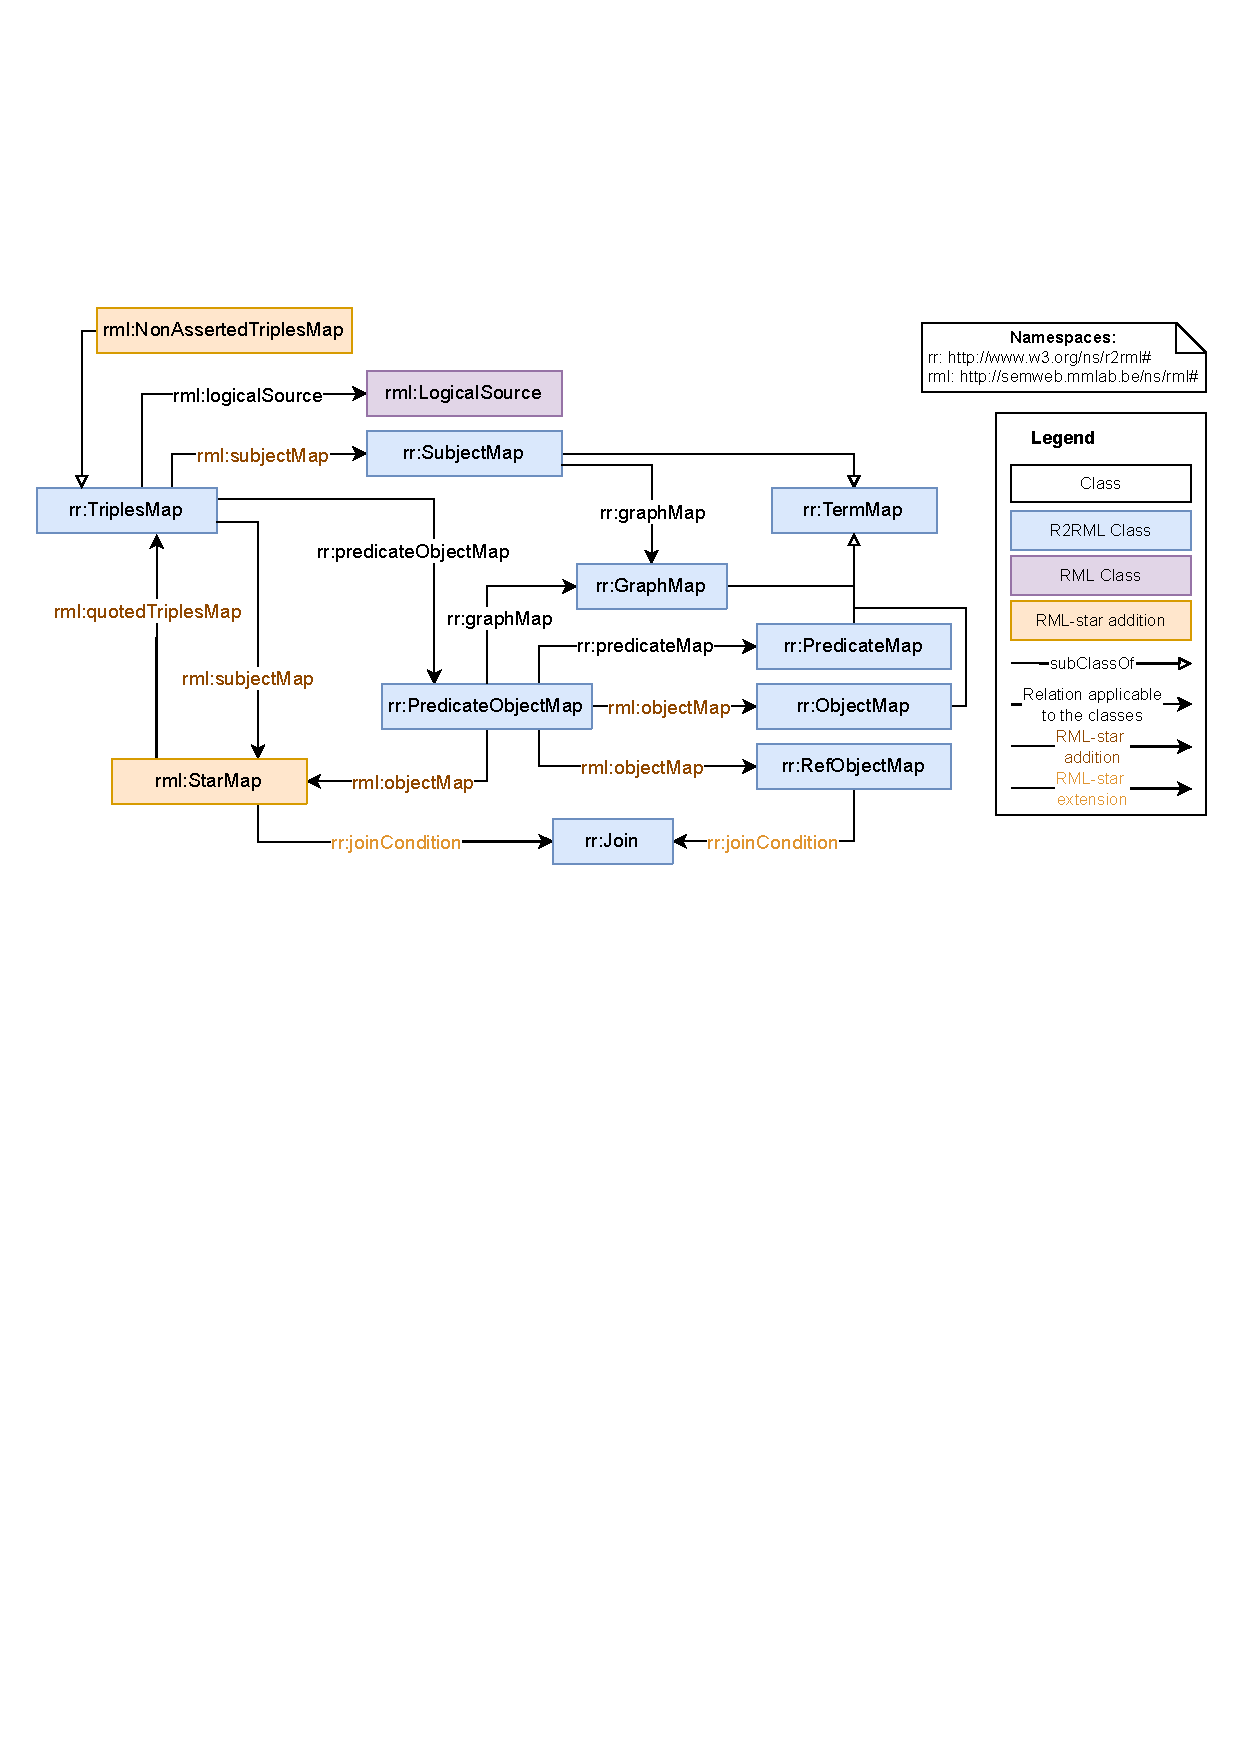
\includegraphics[width=1\linewidth]{figures/rml-star_diagram.pdf}
\caption{The \mbox{RML-star} extension (represented using the Chowlk notation~(\cite{feria2022chowlk})). Orange classes and dark orange object properties show the additions to the RML ontology, light orange object properties represent extensions (i.e., modifications in the domain and/or range).}
\label{fig:rml-star}
\end{figure*}



\subsubsection{Reification with RML-star}

In a previous work~(\cite{delva2021rml-star}), we proposed \mbox{RML-star} (Figure \ref{fig:rml-star}) as an extension of RML to generate \mbox{RDF-star} graphs. 
\mbox{RML-star} adds a new kind of term map, the \texttt{rml:StarMap}, that allows using triples maps to generate quoted triples. Following the \mbox{RDF-star} data model, star maps can only be used in subject and object maps. Star maps use the property \texttt{rml:quotedTriplesMap} to refer to the triples map that generates the quoted triples. This referenced triples map will also generate asserted triples, since it is a \texttt{rr:TriplesMap}. To enable the generation of quoted triples without asserting them, RML-star introduces \texttt{rml:NonAssertedTriplesMap} as a subclass of \texttt{rr:TriplesMap}. Non-asserted triples maps can be referred by \texttt{rml:quotedTriplesMap} to generate quoted triples, but they will be ignored when generating asserted triples.

The \mbox{RML-star} specification~(\cite{iglesias2022rmlstar}) provides a complete description of the language, it is published as a W3C Draft Community Report, and it is maintained by the W3C Knowledge Graph Construction Community Group\footnote{\url{https://www.w3.org/community/kg-construct/}}.
Both, the language and the specification are kept up to date reflecting the modifications in \mbox{RDF-star}.
For instance, the latest \mbox{RML-star} releases update the term ``embedded'' to ``quoted'',
according to the modifications in \mbox{RDF-star}.
%that occurred after the first release of RML-star~\footnote{\url{https://kg-construct.github.io/rml-star-spec/20210706/}}. 
This update renamed the property \texttt{rml:embeddedTriplesMap} to \texttt{rml:quotedTriplesMap}.
An example of an \mbox{RML-star} mapping rule for the data in Listing \ref{lst:csv} is in Listing \ref{lst:rml-star} which generates the \mbox{RDF-star} triples in Listing \ref{lst:res-rml-star}. 
The mapping rules use a non-asserted triples map (\texttt{<\#innerTM>}) within the subject map of a triples map (\texttt{<\#outerTM>}) which annotates quoted triples with \texttt{:date}.


\noindent\hspace{0.19\linewidth}\begin{minipage}{1\linewidth}
\begin{captionedlisting}{lst:rml-star}{Example RML-star mapping that transforms data in Listing \ref{lst:csv}.}
\centering
\begin{tabular}{cc}
\hspace{-7em}{\begin{lstlisting}[basicstyle=\ttfamily\small,label={list:example1},columns=flexible]
<#innerTM> 
  a rml:NonAssertedTriplesMap ;
  rml:logicalSource :marks ;
  rml:subjectMap [ 
    rr:template ":{PERSON}" ] ;
  rr:predicateObjectMap [ 
    rr:predicate :jumps ;
    rml:objectMap [
      rml:reference "MARK" ] ] .
\end{lstlisting}}
&
\hspace{2em}{\begin{lstlisting}[basicstyle=\ttfamily\small,label={list:example1},columns=flexible]
<#outerTM> 
  a rr:TriplesMap ;
  rml:logicalSource :marks ;
  rml:subjectMap [ 
    rml:quotedTriplesMap <#innerTM> ] ;
  rr:predicateObjectMap [ 
    rr:predicate :date ;
    rml:objectMap [
      rml:reference "DATE" ] ] .
\end{lstlisting}}
\end{tabular}
\end{captionedlisting}
\end{minipage}



\noindent\hspace{0.19\linewidth}\begin{minipage}{\linewidth}
\begin{captionedlisting}{lst:res-rml-star}{RDF-star triples generated by the mapping in Listing \ref{lst:rml-star}.}
\centering
\begin{tabular}{c}
\hspace{-1em}
{\begin{lstlisting}[basicstyle=\ttfamily\small,label={list:example1},columns=flexible]
<< :Angelica :jumps "4.80" >> :date "2022-03-21" .
<< :Katerina :jumps "4.85" >> :date "2022-03-19" .
\end{lstlisting}}
\end{tabular}
\end{captionedlisting}
\end{minipage}







\subsection{Validation}
\label{sec:chp4_validation}

We validate \mbox{Morph-KGC$^{star}$} by assessing
1) the engine's conformance with respect to the \mbox{RML-star} specification using \mbox{RML-star} test cases derived from the N-Triples-star syntax tests (Section~\ref{subsec:testcases});
2) its feasibility by applying it in two real-world use cases for software metadata extraction~(\cite{kelley2021framework} (SoMEF)) and biomedical research literature~(\cite{SemMedDB}) (SemMedDB). 
For each use case, we evaluate
a) the generation of triples with \mbox{Morph-KGC$^{star}$} for different reification approaches (Section~\ref{subsubsec:self-comparison}), and 
b) the time performance of \mbox{Morph-KGC$^{star}$} in comparison with the SPARQL-Anything engine~(\cite{daga2021facade,sparql-anything}) to assess our RML-based solution against a SPARQL-based solution (Section~\ref{subsubsec:comparison}).
To the best of our knowledge, SPARQL-Anything is the only open source knowledge graph construction engine able to generate \mbox{RDF-star} datasets apart from \mbox{Morph-KGC$^{star}$}. \ana{revisar este párrafo de intro, porque lo más probable es que elimine toda la parte de sparql-anything, y no haya tantas referencias a morph}


\subsubsection{RML-star Test Cases}

Test cases are commonly used %in standardization processes 
to evaluate the conformance of an engine with respect to a language specification (e.g., RML test cases~(\cite{heyvaert2019conformance})). 
A set of \mbox{RDF-star} test cases was proposed
covering the syntax of various of its serializations\footnote{\url{https://w3c.github.io/rdf-star/tests/}}.
We adapted these test cases
to evaluate the conformance of \mbox{Morph-KGC$^{star}$}
with respect to \mbox{RML-star}.

To create a representative set of test cases for \mbox{RML-star}, we selected the N-Triples-star syntax tests\footnote{\url{https://w3c.github.io/rdf-star/tests/nt/syntax}}, given that \mbox{Morph-KGC$^{star}$} generates the output RDF-star graph in this serialization.  %;and follow a reverse engineering process. 
For each \mbox{RDF-star} test case, we created two associated \mbox{RML-star} test cases that generate the original \mbox{RDF-star} dataset: one test case with a single input data source (i.e., the mapping does not include joins) and another with two input data sources (i.e., the mapping includes joins among triple maps).
For each test case, we manually created the input source(s) in the CSV format and the corresponding \mbox{RML-star} mapping rules to generate the output \mbox{RDF-star} datasets.
Following this approach, we obtained 16 \mbox{RML-star} test cases.
The test cases are openly available at the W3C Community Group on Knowledge Graph Construction~(\cite{david_chaves_2022_6518802}),
and can be reused by any engine to test its conformance with respect to \mbox{RML-star}.
\mbox{Morph-KGC$^{star}$} passes all test cases successfully. As stated in Section \ref{sec:system}, all \mbox{RML-star}, R2RML and RML test cases were added to the continuous integration pipeline of our engine, following best practices in software development.


\subsubsection{Use Cases}

We applied \mbox{Morph-KGC$^{star}$} in two real-world use cases. 
The first generates \mbox{RDF-star} graphs from scientific software documentation, 
and the second annotates statements extracted from biomedical research publications.









%In order to ensure that these results in terms of time are representative, we run each mapping three times and calculate the average time.

%In both use cases we report the time on generating the RDF-star datasets. 




%In summary, our test and use cases show that \mbox{Morph-KGC$^{star}$} generates valid RDF triples and does not add an overhead in the generation time of reified triples. However, a more thorough analysis (out of the scope of this paper) is required to describe the behaviour of each mapping approach.

\noindent\textbf{\textit{Scientific Software Metadata Extraction.}}
Scientific software has become a crucial asset to deliver and reproduce the results described in research publications~(\cite{chue_hong_fair_2021}). However, scientific software is often time consuming to understand and reuse due to incomplete and heterogeneous documentation, available only in a human-readable manner.
The Software Metadata Extraction Framework (SoMEF)~(\cite{somef}) proposes an approach to automatically extract relevant metadata (description, installation instructions, citation, etc.) from code repositories and their documentation. SoMEF includes different text extraction techniques (e.g., supervised classification, regular expressions, etc.) that yield results with different confidence values.
For example, Listing \ref{lst:JSONsnippet} shows a JSON snippet with the description that SoMEF obtained from a software repository (Widoco) using the GitHub API.
The confidence in this case is high as the extracted description was manually curated by the creators of the code repository.
SoMEF extracts more than 30 different metadata fields about 
software, its source code, its released versions, and their corresponding authors. For transforming the output of SoMEF into RDF-star, we used a total of 35 triples maps to annotate software metadata fields and an additional triples map to annotate source code descriptions. All reified triples follow the same structure (Listings \ref{lst:JSONsnippet} \& \ref{lst:TTLsnippet}), i.e. the standard RDF triple contains the excerpt of the extracted feature, and it is annotated
with the \emph{technique} used and the \emph{confidence} value. 
The complete mapping and all input examples and results are available online~(\cite{david_chaves_2022_6919707}).
 
\noindent\hspace{0.1\linewidth}\begin{minipage}{0.8\linewidth}
\begin{captionedlisting}{lst:JSONsnippet}{JSON snippet showing the description metadata field extracted by SoMEF on a code repository using the GitHub API as extraction technique.}
\centering
\hspace{3em}
{
\begin{lstlisting}[basicstyle=\ttfamily\small,label={list:example1},columns=flexible]
"codeRepository": "https://github.com/oeg-upm/Widoco",
"description": [ 
    {
      "confidence": [
        1.0
      ],
      "excerpt": "Wizard for documenting ontologies. WIDOCO is ...",
      "technique": "GitHub API"
    }
  ]  
\end{lstlisting}
}
\end{captionedlisting}
\end{minipage}

Capturing the technique used and the confidence obtained for each extracted metadata field is key for obtaining an accurate representation of the result. Hence, the \mbox{RDF-star} representation corresponding to the JSON in Listing \ref{lst:JSONsnippet} includes this information, as depicted in Listing \ref{lst:TTLsnippet}.

%\begin{minipage}{0.9\linewidth}
%\begin{captionedlisting}{lst:TTLsnippet}{N-Triples-star snippet showing the results generated for the %description field shown in Listing \ref{lst:JSONsnippet}. Each asserted triple is annotated with its %corresponding confidence and technique.}
%\centering
%\begin{tabular}{c}
%\hspace{1.4em}
%{
%\begin{lstlisting}[numbers=left]
%<< <https://example.org/oeg-upm/Widoco> <https://w3id.org/okn/o/sd#description> 
%    "Wizard for documenting ontologies. WIDOCO is ..." >> 
%        <https://www.w3id.org/okn/o/em#technique> "GitHub API" .
%<< <https://example.org/oeg-upm/Widoco> <https://w3id.org/okn/o/sd#description> 
%    "Wizard for documenting ontologies. WIDOCO is ..." >> 
%        <https://www.w3id.org/okn/o/em#confidence> "1.0" .
%<https://example.org/oeg-upm/Widoco> <https://w3id.org/okn/o/sd#description> 
%    "Wizard for documenting ontologies. WIDOCO is ..." .
%\end{lstlisting}
%}
%\end{tabular}
%\end{captionedlisting}
%\end{minipage}        


\begin{captionedlisting}{lst:TTLsnippet}{RDF-star triples snippet showing the results generated for the description field in Listing \ref{lst:JSONsnippet}. Each asserted triple is annotated with its corresponding confidence and technique.}
\centering
{
\begin{lstlisting}[basicstyle=\ttfamily\small,label={list:example1},columns=flexible]
ex:oeg-upm/Widoco :description "Wizard for documenting ontologies. WIDOCO is ..." .
<<ex:oeg-upm/Widoco :description "Wizard for documenting ontologies. WIDOCO is ...">> 
    :technique "GitHub API" .
<<ex:oeg-upm/Widoco :description "Wizard for documenting ontologies. WIDOCO is ...">> 
    :confidence "1.0" .
\end{lstlisting}
}
\end{captionedlisting}


%For example, for \cref{lst:JSONsnippet}, the excerpt of the software's description ("Wizard for documenting ontologies. WIDOCO is ...") was extracted with the technique "GitHub API" with a confidence of 1.0. 
% talk about the execution
%The reified triples are used for describing the software, that uses


\noindent\textbf{\textit{Biomedical Research Literature.}} 
SemMedDB~(\cite{SemMedDB}), the Semantic MEDLINE Database, is a repository 
that contains information on extracted biomedical entities 
and predications (subject-predicate-object triples) 
from biomedical texts (titles and abstracts from PubMed citations). 
%consists of a set of triples and annotations automatically extracted from PubMed titles, abstracts, and citations. 
%a set of data sources with automatic semantic annotations from titles and abstracts of citations available in PubMed.
The tables comprising SemMedDB are available for download as a relational database or CSV files\footnote{ \url{https://lhncbc.nlm.nih.gov/ii/tools/SemRep_SemMedDB_SKR/SemMedDB_download.html}}.
We downloaded the MySQL files for (1)~predication predictions (PREDICATION and PREDICATION\_AUX tables), containing more than 117 million annotations; and (2)~entity predictions (ENTITY table), which include more than 410 million annotations.
Listings \ref{lst:semmeddb_entity}, \ref{lst:semmeddb_pred} and \ref{lst:semmeddb_predaux} illustrate the columns used from the tables with synthetic data. 
For predications, only data for subjects is shown; the missing columns regarding objects follow the same structure as subjects.
%This data contains information on predicted entities and predicted subject-predicate-object predications.
Subjects and objects, from predications, and entities are assigned a semantic type 
(that categorizes the extracted concept in the biomedical domain) annotated with a confidence score. 
In addition, the extraction of subjects and objects is assigned a timestamp on when it took place. 
Thus, the score and timestamp represent metadata about other statements.
We created an RML-star mapping with 5 triples maps quoting triples:
3 of them are used to annotate the assignation of semantic types to entities, subjects, and objects with confidence scores;
the remaining 2 provide the timestamps for the extraction of subjects and objects. 

\begin{minipage}{0.38\linewidth}
\begin{captionedlisting}{lst:semmeddb_entity}{ENTITY table snippet.}
\centering
\begin{tabular}{c}
\hspace{-1em}
{
\begin{lstlisting}[basicstyle=\ttfamily\small,label={list:example1},columns=flexible]
ENTITY_ID , SEMTYPE , SCORE
12345        , orga        , 790
\end{lstlisting}
}
\end{tabular}
\end{captionedlisting}
\end{minipage}
\,\,\,\,\hfill
\begin{minipage}{0.6\linewidth}
\begin{captionedlisting}{lst:semmeddb_pred}{PREDICATION table snippet.}
\centering
\begin{tabular}{c}
\hspace{-1em}
{
\begin{lstlisting}[basicstyle=\ttfamily\small,label={list:example1},columns=flexible]
PREDICATION_ID , SUBJECT_SEMTYPE , SUBJECT_NAME
13579               , Semtype               , SubjName
\end{lstlisting}
}
\end{tabular}
\end{captionedlisting}
\end{minipage}

\noindent\hspace{0.23\linewidth}\begin{minipage}{0.8\linewidth}
\begin{captionedlisting}{lst:semmeddb_predaux}{PREDICATION\_AUX table snippet.}
\centering
\begin{tabular}{c}
\hspace{-7em}
{
\begin{lstlisting}[basicstyle=\ttfamily\small,label={list:example1},columns=flexible]
PREDICATION_AUX_ID, PREDICATION_ID, SUBJECT_SCORE, TIMESTAMP
67890                   , 13579              , 800               , 1651740766
\end{lstlisting}
}
\end{tabular}
\end{captionedlisting}
\end{minipage}

\noindent\hspace{0.1\linewidth}\begin{minipage}{0.78\linewidth}
\begin{captionedlisting}{lst:semmeddb_triples}{RDF-star triples generated from data in Listings \ref{lst:semmeddb_entity}, \ref{lst:semmeddb_pred} and \ref{lst:semmeddb_predaux}.}
\centering
\begin{tabular}{c}
\hspace{-1.5em}
{
\begin{lstlisting}[basicstyle=\ttfamily\small,label={list:example1},columns=flexible]
<<ex:12345 sem:semanticType "orga">> sem:score "790" .
<<ex:13579 sem:subject ex:SubjName>> sem:timestamp "1651740766" .
<<ex:SubjName sem:semanticType "Semtype">> sem:score "800" .
\end{lstlisting}
}
\end{tabular}
\end{captionedlisting}
\end{minipage}
